%-------------------------------------------------------------------------------
% yum_kitedit
%-------------------------------------------------------------------------------
%
% \file        yum_kitedit.tex
% \library     Documents
% \author      Chris Ahlstrom
% \date        2015-06-07
% \update      2016-12-22
% \version     $Revision$
% \license     $XPC_GPL_LICENSE$
%
%     Provides the Kit section of yoshimi-user-manual.tex.
%
%-------------------------------------------------------------------------------

\section{Kit Edit}
\label{sec:kit_edit}

   The \textsl{Yoshimi} Kit dialog is a dialog for creating a
   set of drums or layered instruments.
   It provides a way to use individual voices and synth blocks to create
   drumlike sounds, or complex layered sounds.
   Within this window one can create drum kits, layered instruments, or one
   can combine more instruments into one instrument.  

   Is this true of \textsl{Yoshimi}?:

   Item 0 is a special type: it cannot be disabled (but it can be muted), to
   edit it one must use "ADs edit" or "SUBs edit" from the part window.

\begin{figure}[H]
   \centering 
   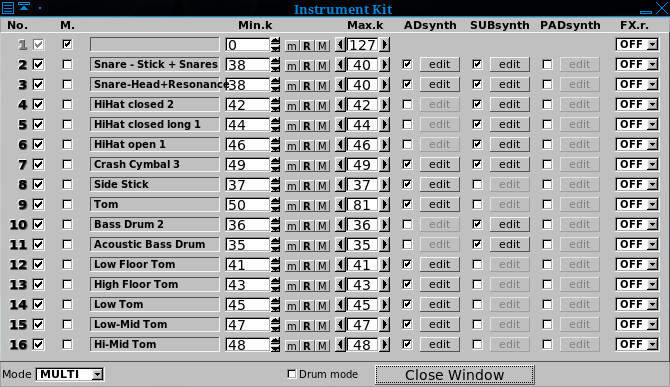
\includegraphics[scale=1.0]{bottom-panel/instrument-edit/Kit/instrument-kit-edit.jpg}
   \caption{Kit Edit Dialog}
   \label{fig:kit_edit_dialog}
\end{figure}

   \begin{enumber}
      \item \textbf{Rows 1 to 16.}
         This dialog contains 16 identical rows containing the following
         elements, in the order given:
         \begin{enumber}
            \item \textbf{No.}
            \item \textbf{Enable}
            \item \textbf{M.}
            \item \textbf{Instrument Name}
            \item \textbf{Min.k}
            \item \textbf{m} (set minimum note)
            \item \textbf{R} (reset default note range)
            \item \textbf{M} (set maximum note)
            \item \textbf{Max.k}
            \item \textbf{ADsynth}
               \begin{enumber}
                  \item \textbf{Enable}
                  \item \textbf{edit}
               \end{enumber}
            \item \textbf{SUBsynth}
               \begin{enumber}
                  \item \textbf{Enable}
                  \item \textbf{edit}
               \end{enumber}
            \item \textbf{PADsynth}
               \begin{enumber}
                  \item \textbf{Enable}
                  \item \textbf{edit}
               \end{enumber}
            \item \textbf{FX.r}
         \end{enumber}
      \item \textbf{Mode}
      \item \textbf{Drum mode}
      \item \textbf{Close Window}
   \end{enumber}

   Some items described in ZynAddSubFX that aren't seen in any diagrams:

   \begin{enumber}
      \item Kit Mode. Enable the kit mode.
      \item Protect the kit. when loading an instrument, only item 0 will be
      changed,
      Other items will remain untouched. This allows one to combine more
      instruments. If one wants to add more instruments to the kit, one must
      copy the item 0 to another item, because the item 0 will be replaced. If
      one loads master settings or clearx the instrument/master setting,
      the kit is cleared .
      \item Swap/Copy. Swap two items or copy a item to other item.
   \end{enumber}

   \setcounter{ItemCounter}{0}      % Reset the ItemCounter for this list.

   \itempar{No}{kit!row number}
   Kit Row Number.
   Kit Item Number.
   A simple label to indicate the instrument number in the kit.

   \itempar{Enable}{kit!enable}
   Kit Row Enable.

   Value: \texttt{Off*, On}

   \itempar{M}{kit!M.}
   Kit Row "M".
   Mute an item of the kit.

   \itempar{Instrument Name}{kit!name}
   Kit Instrument Name.

   \itempar{Min.k}{kit!minimum key}
   Kit Instrument Minimum Key.
   Sets the minimum key of the item of the kit.

   \itempar{m}{kit!m}
   Sets the minimum note of this instrument to value of the last note
   pressed.

   \itempar{R}{kit!R}
   Resets the minimum and maximum notes to their default values.

   \itempar{M}{kit!M}
   Sets the maximum note of this instrument to value of the last note
   pressed.

   \itempar{Max.k}{kit!maximum key}
   Kit Instrument Maximum Key.
   Sets the maximum key of the item of the kit.

   \itempar{ADsynth}{kit!addsynth}
   Kit ADDsynth.
   A checkbox is provided to enable/disable this synth component, and
   an edit button is provided to edit the component.

   \itempar{SUBsynth}{kit!subsynth}
   Kit SUBsynth.
   A checkbox is provided to enable/disable this synth component, and
   an edit button is provided to edit the component.

   \itempar{PADsynth}{kit!padsynth}
   Kit PADsynth.
   A checkbox is provided to enable/disable this synth component, and
   an edit button is provided to edit the component.

   \itempar{FX.r}{kit!fx.r}
   Kit Effect.
   Chooses the Part Effect (PartFX) to process the item (OFF means that is
   unprocessed). 

   Values: \texttt{OFF, FX1, FX2, FX3}

   \itempar{Mode}{kit!mode}
   Kit Mode.

   We need a picture to show the full \textbf{Mode} menu.

   \index{kit!mode off}
   \index{kit!mode single}
   \index{kit!mode multi}
   \index{kit!mode crossfade}
   \begin{itemize}
      \item \textbf{Off} means no kit is enabled, so one only has the Add,
         Sub, and Pad sounds in the Instrument Edit window.
      \item \textbf{Multi} means all the kit items will sound together
         regardless of their note ranges.
      \item \textbf{Single} means only the lowest numbered item will sound
         in a given note range. There will be no overlap.
      \item \textbf{Crossfade} is described in detail below.
   \end{itemize}

   For example:
   Item 0 has \textbf{Min.k} set to 0 and \textbf{Max.k} set to 60, and
   Item 1 has \textbf{Min.k} set to 40 and \textbf{Max.k} set to 127.

   \index{kit!mode single}
   In \textbf{SINGLE mode}, only Item 0 will sound in the note range 0 to
   60, and Item 1 will sound in the range 61 to 127.

   \index{kit!mode multi}
   In \textbf{MULTI} mode, only Item 0 will sound in the range 0 to 40, both
   items will sound from 41 to 60, and only Item 1 will sound from 61 to
   127.

   Values: \texttt{OFF*, MULTI, SINGLE}.

   \index{kit!mode crossfade}
   The part's kit edit \textbf{Mode} menu has an extra entry
   called \textbf{Crossfade}.
   When cross-fade is set, one gets Multi behaviour with overlapping key
   ranges, but with a very smooth cross-fade between sequential \textsl{pairs}
   of kit items. This follows the pattern 1+2, 3+4, etc. Each pair will not
   affect any other kit items.

   It doesn't matter which of the pair has the lower range, as long as there is
   a range overlap. The code is semi-intelligent, and any that are not paired
   will exhibit normal Multi behaviour. If one item in a pair is not enabled
   then the other one will exhibit normal Multi behaviour and will not fade at
   all.

   An interesting effect is that if one of the pair is enabled, but muted or
   has no engines enabled, then the other one still fades through the overlap
   range, so one can get sounds fading out (or fading in) with increasing
   pitch!

   If one wants a fade to come in then go out again, one needs two sets of pairs,
   with a hard non-overlapped point in the middle.

   \begin{verbatim}
   item 1 - min 0 max 60
   item 2 - min 40 max 80 (fades up)
   \end{verbatim}

   \begin{verbatim}
   item 3 - min 81 max 100 (fades down)
   item 4 - min 90 max 127
   \end{verbatim}

   This feature is backward-compatible, in that older versions of
   \textsl{Yoshimi} will
   see it as an ordinary Multi -- it uses a new variable stored in the
   instrument file that is simply ignored by earlier versions.

   \itempar{Drum mode}{kit!drum mode}
   Kit Drum Mode.
   If drum-mode  is set, then microtonal tuning is ignored for this kit,
   otherwise it could make drum sounds very unpredictable!

   \itempar{Close Window}{kit!close}
   Close.

%-------------------------------------------------------------------------------
% vim: ts=3 sw=3 et ft=tex
%-------------------------------------------------------------------------------
